% =====================================================================
% Snippet: mini-spectrogram.tex
% =====================================================================
% USAGE: Mini mel-spectrogram (time × frequency heatmap) with axis
% labels. For audio/speech architecture figures (Whisper, Tacotron).
%
% Copy %% COPY-START / END, replace:
%   - cell sizes, dimensions
%   - n_time, n_freq: # cells in each axis
%   - color gradient: cellLo / cellHi
%   - origin
% =====================================================================

\documentclass[tikz,border=10pt]{standalone}
\usepackage{xcolor,tikz}
\usetikzlibrary{positioning,calc}

\definecolor{specLo}{HTML}{EEF3F8}
\definecolor{specMid}{HTML}{5AB8B8}
\definecolor{specHi}{HTML}{1F8F8F}
\definecolor{acaTealLine}{HTML}{1F8F8F}
\definecolor{acaGreyLine}{HTML}{606060}

\begin{document}
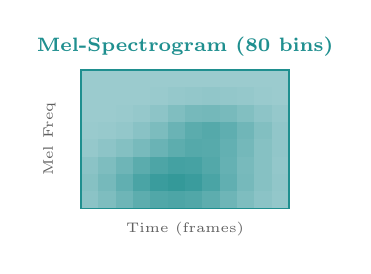
\begin{tikzpicture}

%% COPY-START =========================================================

\def\xO{0}
\def\yO{0}
\def\nTime{12}        % time bins (x-axis)
\def\nFreq{8}         % frequency bins (y-axis, mel)
\def\cellW{0.22}      % cell width
\def\cellH{0.22}      % cell height

% --- CELLS: realistic mel-spec pattern (formants + harmonics) ---
% Pattern: low freq energetic, mid-time vowel resonance, decays in high freq
\foreach \i in {1,...,\nFreq} {
  \foreach \j in {1,...,\nTime} {
    % Formant-like pattern: high at low freq + mid time
    \pgfmathsetmacro\val{
      40 + 50 * exp(-((\i - 2)/2)^2 - ((\j - 6)/4)^2)
      + 30 * exp(-((\i - 5)/1.5)^2 - ((\j - 8)/3)^2)
    }
    \pgfmathsetmacro\val{int(min(95, max(15, \val)))}
    \pgfmathsetmacro\cx{\xO + (\j - 0.5) * \cellW}
    \pgfmathsetmacro\cy{\yO + (\i - 0.5) * \cellH}
    \fill[specHi!\val!specLo]
      (\cx - \cellW/2, \cy - \cellH/2) rectangle
      (\cx + \cellW/2, \cy + \cellH/2);
  }
}

% --- BORDER ---
\draw[acaTealLine, line width=0.5pt]
  (\xO, \yO) rectangle
  (\xO + \nTime * \cellW, \yO + \nFreq * \cellH);

% --- Y-AXIS LABEL (Freq, mel) ---
\node[anchor=south, font=\tiny, color=acaGreyLine, rotate=90]
  at (\xO - 0.2, \yO + \nFreq * \cellH / 2)
  {Mel Freq};

% --- X-AXIS LABEL (Time) ---
\node[anchor=north, font=\tiny, color=acaGreyLine]
  at (\xO + \nTime * \cellW / 2, \yO - 0.05)
  {Time (frames)};

% --- TITLE ---
\node[anchor=south, font=\scriptsize\bfseries, color=acaTealLine]
  at (\xO + \nTime * \cellW / 2, \yO + \nFreq * \cellH + 0.05)
  {Mel-Spectrogram (80 bins)};

%% COPY-END ===========================================================

\end{tikzpicture}
\end{document}
